\pdfsuppresswarningpagegroup=1
\section{Results - data not fitted}
\paragraph{Note}{Do we want results in and out of sample? Still don't
fully understand in sample results. Need to add finite replica/fit results}

Also need to define list of datasets and new vs old processes

\subsection{Data space estimators}

\paragraph{Note}{Add bias and variance across fits to show respective spreads}

First we show $\sqrt{\frac{\eshift{\bias}}{\eshift{\var}}}$ by experiment for data
not included in the fit, but old processes.

\begin{center}
    \begin{tabular}{lrr}
        \toprule
        {} &  $\ndata$ &  $\sqrt{\frac{\eshift{\bias}}{\eshift{\var}}}$ \\
        experiment &        &                      \\
        \midrule
        HERACOMB   &     63 &                 1.60 \\
        ATLAS      &    371 &                 0.76 \\
        CMS        &    310 &                 0.87 \\
        LHCb       &     35 &                 0.83 \\
        Total      &    779 &                 0.89 \\
        \bottomrule
        \end{tabular}
\end{center}

Next we show the same estimator, $\sqrt{\frac{\eshift{\bias}}{\eshift{\var}}}$, by
experiment for data not included in the fit, new processes

\begin{center}
    \begin{tabular}{lrr}
        \toprule
        {} &  $\ndata$ &  $\sqrt{\frac{\eshift{\bias}}{\eshift{\var}}}$ \\
        experiment &        &                      \\
        \midrule
        ATLAS      &    374 &                 1.00 \\
        CMS        &    179 &                 0.81 \\
        Total      &    553 &                 0.90 \\
        \bottomrule
        \end{tabular}
\end{center}

Now we compare the measured $\xi_{1\sigma}$ and estimated $\xi_{1\sigma}$ by experiment
for data not included in the fit, old processes. To estimate $\xi_{1\sigma}$
we we take $\sqrt{\frac{\eshift{\bias}}{\eshift{\var}}}$ and substitute into
eq. \eqref{eq:expectedxi}, assuming that $\frac{\sigma_i}{\modelstd_i}$ is
constant across datapoints and equal to $\sqrt{\frac{\eshift{\bias}}{\eshift{\var}}}$.

\begin{center}
    \begin{tabular}{lrrr}
        \toprule
        {} &  $\ndata$ &  measured $\xi_{1\sigma}$ &  estimated $\xi_{1\sigma}$ from bias/variance \\
        experiment &        &                           &                                                  \\
        \midrule
        HERACOMB   &     63 &                      0.46 &                                             0.47 \\
        ATLAS      &    371 &                      0.77 &                                             0.81 \\
        CMS        &    310 &                      0.69 &                                             0.75 \\
        LHCb       &     35 &                      0.78 &                                             0.77 \\
        Total      &    779 &                      0.72 &                                             0.74 \\
        \bottomrule
        \end{tabular}
\end{center}


Similarly, we compare the same estimators $\xi_{1\sigma}$ and estimated
$\xi_{1\sigma}$ by experiment for data not included in the fit, new processes.

\begin{center}
    \begin{tabular}{lrrr}
        \toprule
        {} &  $\ndata$ &  measured $\xi_{1\sigma}$ &  estimated $\xi_{1\sigma}$ from bias/variance \\
        experiment &        &                           &                                                  \\
        \midrule
        ATLAS      &    374 &                      0.66 &                                             0.69 \\
        CMS        &    179 &                      0.76 &                                             0.78 \\
        Total      &    553 &                      0.69 &                                             0.73 \\
        \bottomrule
        \end{tabular}
\end{center}


We now show $\xi_{1\sigma}^{i}$ for data which was not fitted, old processes. Split
up by experiment, each scatter point is $\xi_{1\sigma}^{i}$ for a given datapoint
in the basis which diagonalises the respective experimental covariance matrix.

\begin{figure}[!b]
    \centering
    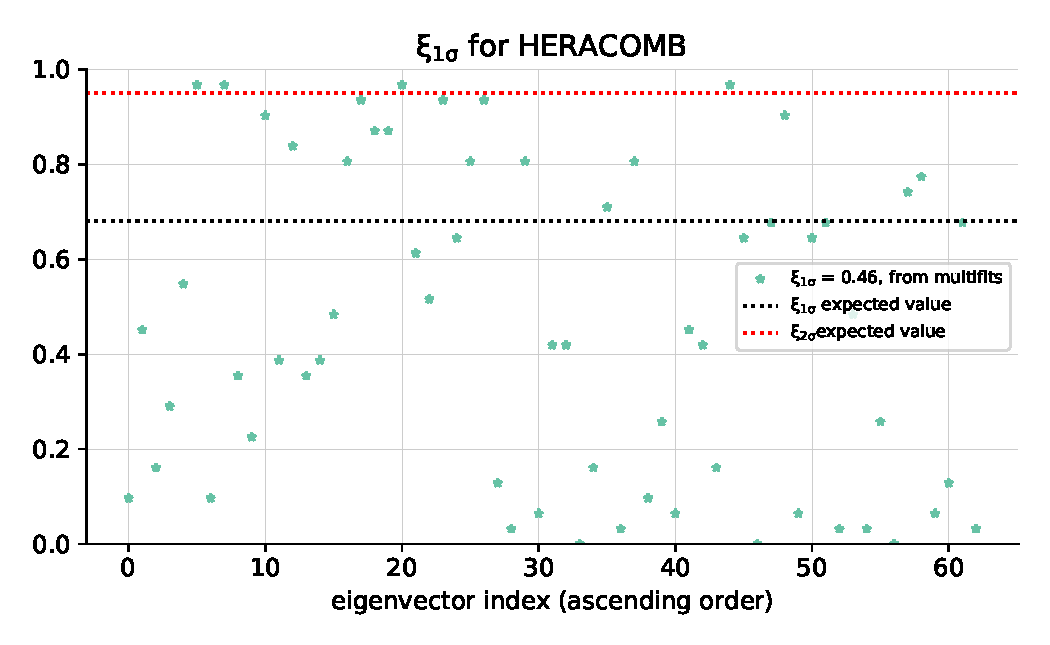
\includegraphics[width=0.6 \textwidth]{out_oldproc_hera_xi.pdf}
    \caption{$\xi_{1\sigma}^{i}$ for HERA datasets which were not fitted
    but are old processes, in the basis which diagonalises the experimental
    covariance matrix}
    \label{fig:outoldheraxi}
\end{figure}

\begin{figure}[ht]
    \centering
    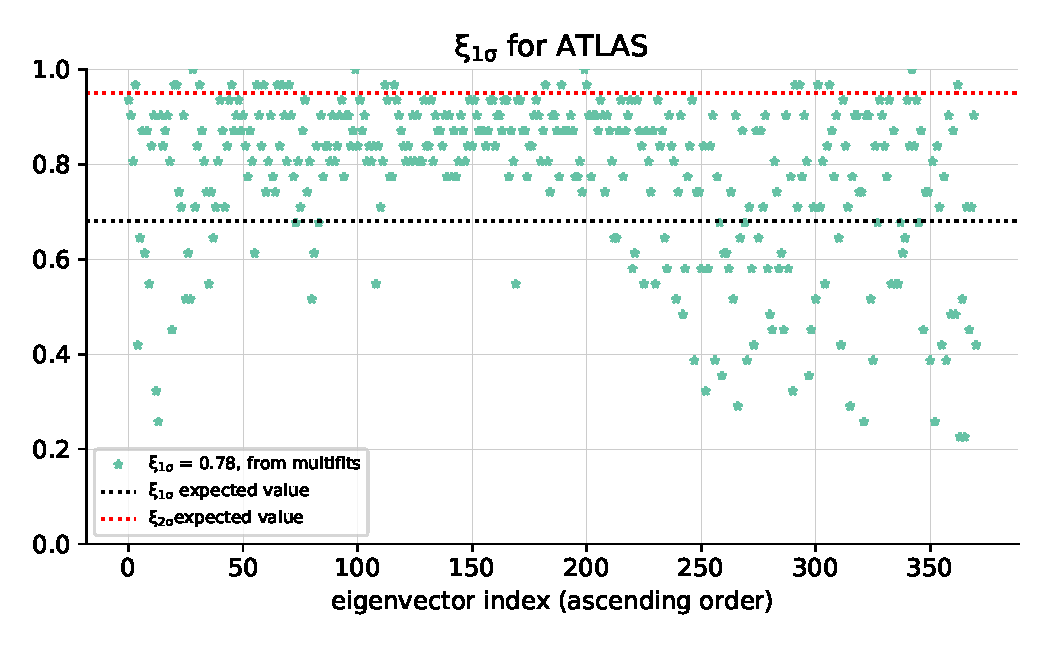
\includegraphics[width=0.6 \textwidth]{out_oldproc_atlas_xi.pdf}
    \caption{$\xi_{1\sigma}^{i}$ for ATLAS datasets which were not fitted
    but are old processes, in the basis which diagonalises the experimental
    covariance matrix}
    \label{fig:outoldatlasxi}
\end{figure}

\begin{figure}[ht]
    \centering
    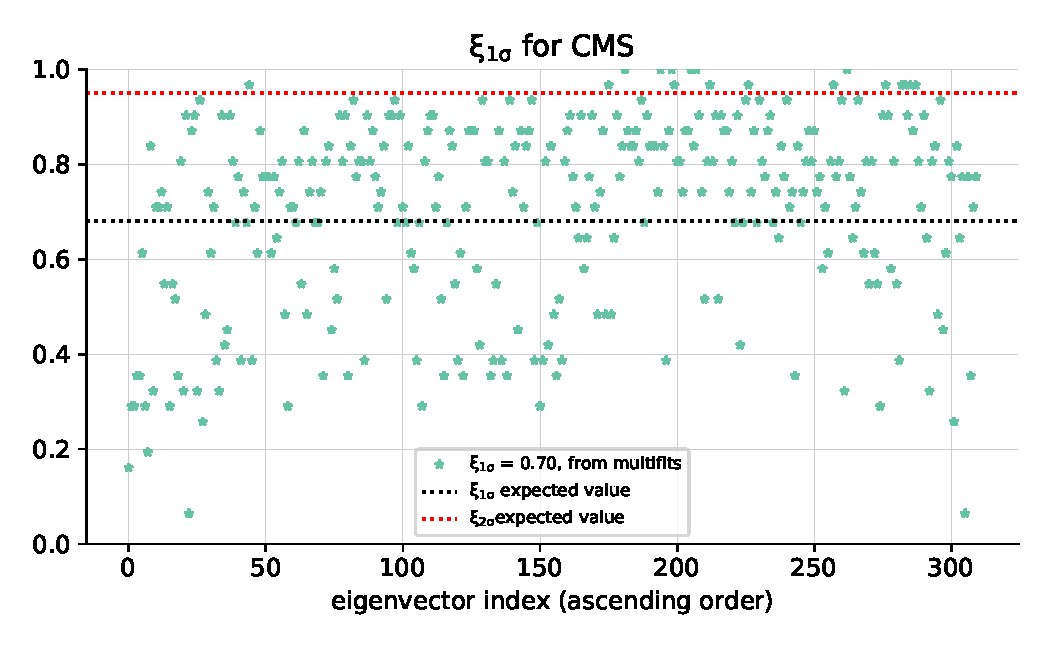
\includegraphics[width=0.6 \textwidth]{out_oldproc_cms_xi.pdf}
    \caption{$\xi_{1\sigma}^{i}$ for CMS datasets which were not fitted
    but are old processes, in the basis which diagonalises the experimental
    covariance matrix}
    \label{fig:outoldcmsxi}
\end{figure}

\begin{figure}[ht]
    \centering
    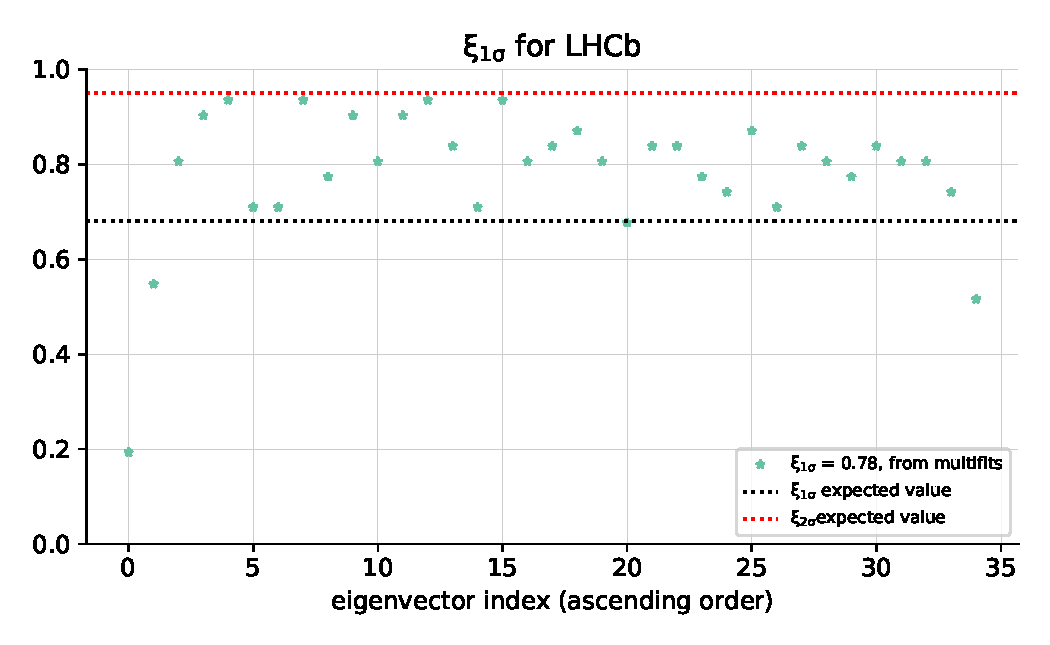
\includegraphics[width=0.6 \textwidth]{out_oldproc_lhcb_xi.pdf}
    \caption{$\xi_{1\sigma}^{i}$ for LHCb datasets which were not fitted
    but are old processes, in the basis which diagonalises the experimental
    covariance matrix}
    \label{fig:outoldlhcbxi}
\end{figure}

Now the corresponding plots for data which was not fitted, new processes.

\begin{figure}[ht]
    \centering
    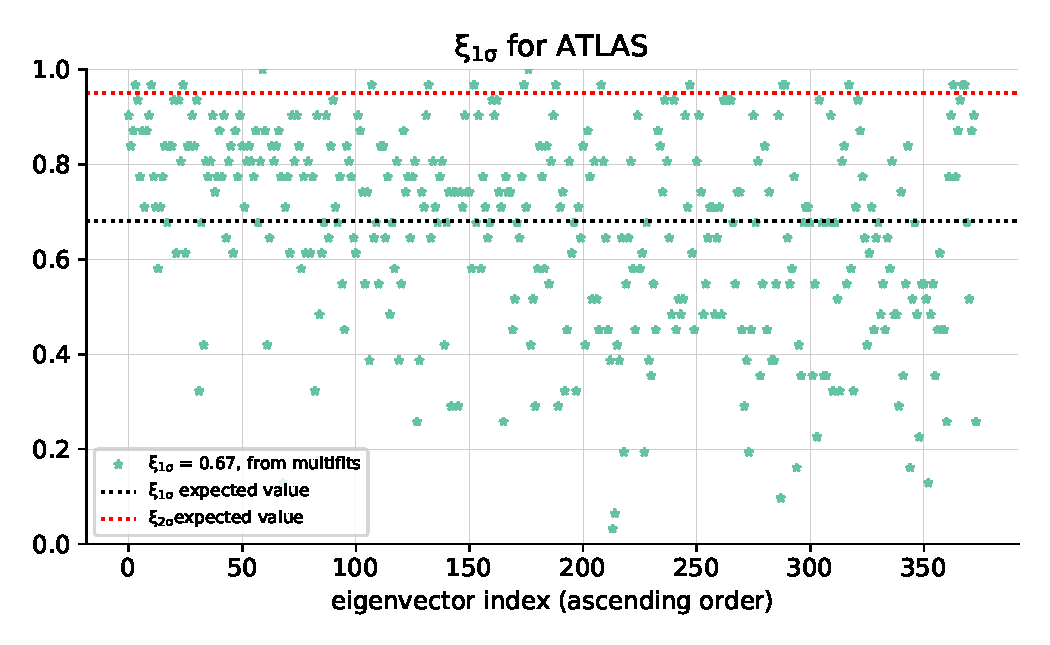
\includegraphics[width=0.6 \textwidth]{out_newproc_atlas_xi.pdf}
    \caption{$\xi_{1\sigma}^{i}$ for ATLAS datasets which were not fitted
    and are new processes, in the basis which diagonalises the experimental
    covariance matrix}
    \label{fig:outnewatlasxi}
\end{figure}

\begin{figure}[ht]
    \centering
    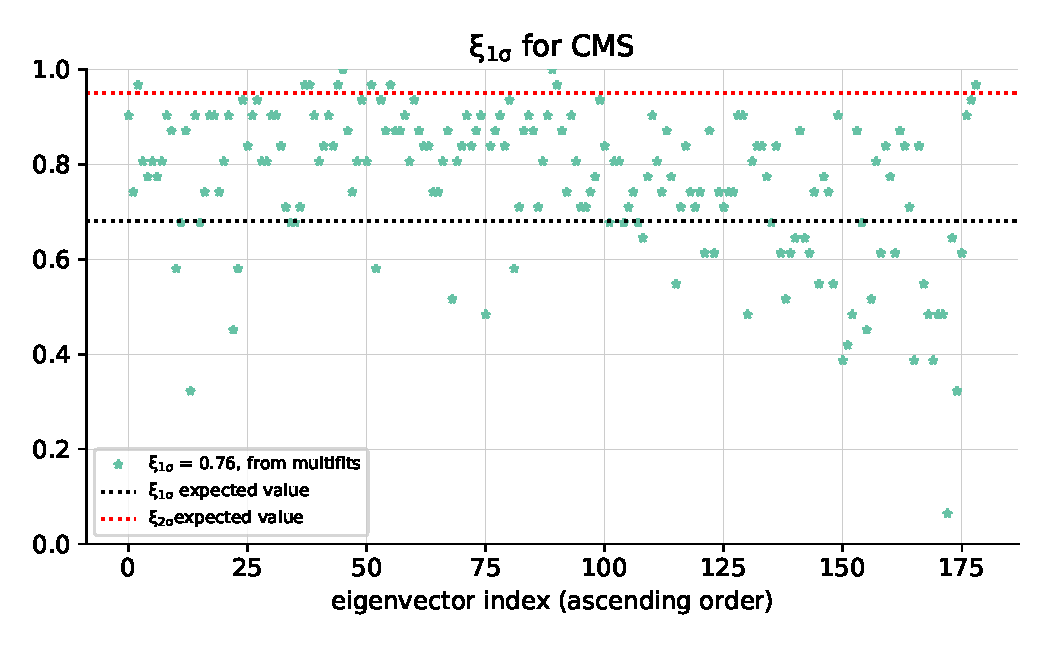
\includegraphics[width=0.6 \textwidth]{out_newproc_cms_xi.pdf}
    \caption{$\xi_{1\sigma}^{i}$ for CMS datasets which were not fitted
    and are new processes, in the basis which diagonalises the experimental
    covariance matrix}
    \label{fig:outnewcmsxi}
\end{figure}

There is no noticeable trend between new and old processes with the data which
was not fitted. Potentially we can condense the above plots significantly. At
least into just 4 plots (by experiment). The results would change slightly
due to the basis being different.
